\chapter{Introducci\'{o}n y Objetivos}
\label{chap:intro}
\graphicspath{{../figs/chap_intro/}} 

%********************************************************************************************************
\section{Motivaci\'{o}n}
\label{sec:sec1}

Esto es una sección.
Puedes referenciar la Sección \ref{sec:sec1} o la subsección \ref{sec:subsec} de esta manera.
También se pueden referenciar diferentes citas bibliográficas \citep{ExArt01,ExIncollec01,ExInpro01,ExTech01,ExBook01,ExPHD01}.
Referenciamos una figura \ref{fig:fig1}. 
Esta es la primera vez que aparece un acrónimo \gls{pv} y luego esta es la segunda vez que aparece, \gls{pv}. \mnote{Photovoltaic}

\begin{figure}[htb]
	\centering
	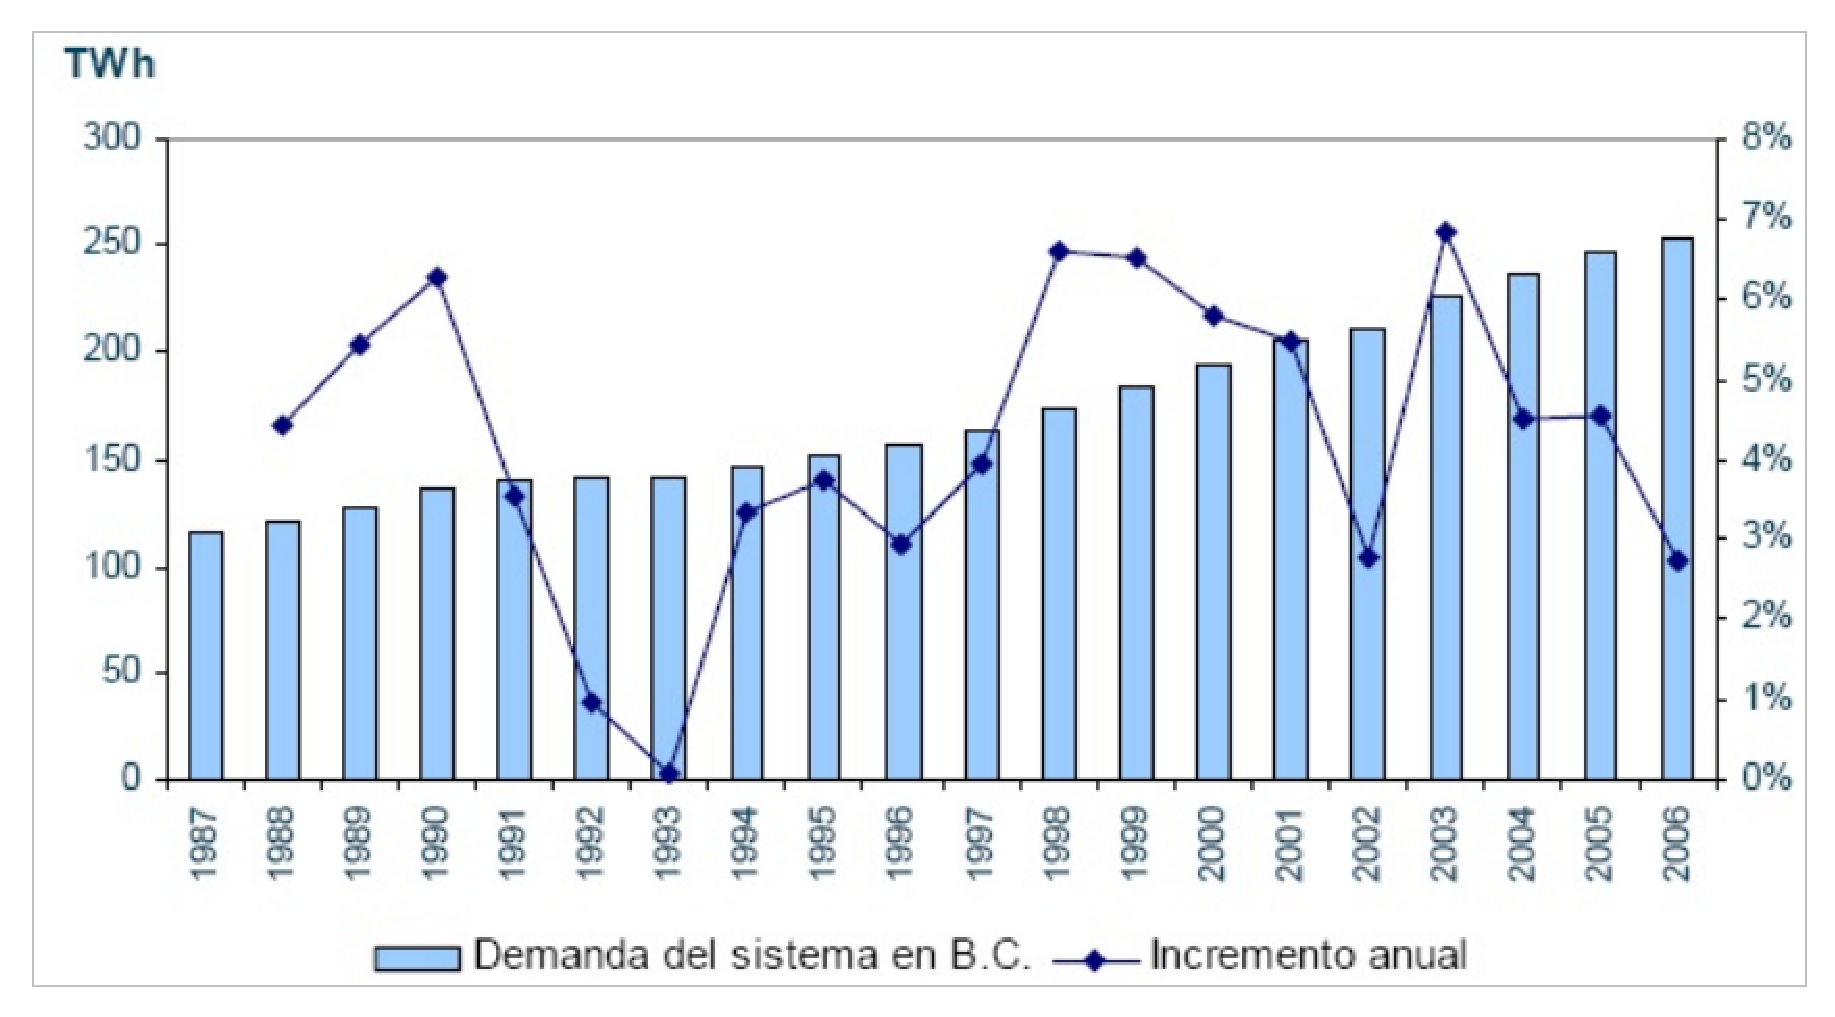
\includegraphics[width=0.9\textwidth]{creci_dem.eps} 
  \caption[Descripción corta para el índice]
  {Pie de foto debajo de la figura.}
	\label{fig:fig1}                                               
\end{figure}

%--------------------------------------------------------------------------------------------------------
\subsection{La demanda el\'{e}ctrica en España}
\label{sec:subsec}

Esto es una subsección. 
Podemos referenciar una Ecuación \ref{eq:ctrnn}.

\begin{equation}
  \begin{array}{l}
    \dot y_{i}(t)= f_i(y_1(t),y_2(t)) = \\ 
    = \frac{1}{\tau_i}\cdot\left(-y_i(t)+\sum_{j=1}^2w_{ij}\cdot \varphi\left(y_j(t)+\theta_j\right)+x_i(t)\right) \\\\
    with\;\varphi(x)=\frac{1}{1+e^{-x}}\;\;and\;\;i=1,2.
  \end{array}
  \label{eq:ctrnn}
\end{equation}

Tenemos una lista de elementos:
\begin{itemize}
  \item Elemento 1: Hacemos una referencia bibliográfica \citep{ExArt01}.
  \item Elemento 2: Elemento matemático $\phi_i(x)$.
\end{itemize}

O podemos referenciar incluso una Tabla \ref{tab:table1}

\begin{table}[!t]
  \centering
  \resizebox{0.75\textwidth}{!}{%
  \begin{tabular}{lcc} \toprule
    \multirow{2}{*}{Electrodomésticos} & Consumo & Porcentaje del total \\ 
                                       & (Wh/day)& (\%)           \\ \midrule
    \multicolumn{3}{l}{\emph{Diferible}} \\
    Lavadora            & 785.92      & 6.95 \\ 
    Secadora            & 962.6       & 8.5  \\
    Lavavajillas        & 693.6       & 6.13 \\
    Total (diferible)   & 2442.12     & 21.6 \\ \midrule
    \multicolumn{3}{l}{\emph{No diferible}}     \\
    Luces                & 1302        & 11.5   \\
    Horno                & 1255.15     & 11.1   \\
    Frigorífico          & 616.73      & 5.4    \\
    Ordenador y          &             &        \\
    electrónica de       & 5694        & 50.03  \\  
    consumo (TV,DVD,etc.)&             &        \\
    Total (No diferible) & 8867.88     & 78.4   \\ \midrule
    Total                & 11310       & 100    \\ \bottomrule
  \end{tabular}}
  \caption[Descripción corta de la tabla para el índice.]
  {Pie de tabla.}
  \label{tab:table1}
\end{table}
